%Sidenote from Angie: Green text after a percentage sign includes notes to the LaTeX code, useful tips and tricks I thought you might need ⁠— feel free to read them for extra info on this template.

%~~~~~~~~~~~~~~~~~~~~~~~~~~~~~~~~~~~~~~~~~~~~~~~~~~~~~~~%
% Changelog 7.21: Lab now moving from remote learning to physical laboratory, please ignore any comments after '% OLD TEXT IGNORE:'
%Changelog 10.21: Fixed the formatting of RSC referencing style 
%Changelog 1.22: Reviewed before the start of Semester 2, fixed some wording/clarification issues
%Changelog 5.22: Reviewed after semester 2, fixed some wording/clarification issues, removed OLD TEXT
%~~~~~~~~~~~~~~~~~~~~~~~~~~~~~~~~~~~~~~~~~~~~~~~~~~~~~~~%

\documentclass[twocolumn]{article} %sets the type of the document that you compile, for just now it is an article - specifically one with a two-column formatting

%~~~~~~~ Packages ~~~~~~~~~%
% Please don't be scared by the chunk of code below, these are just some handy tools that make using LaTeX easier, you can read more on your own time, for example here: https://www.latex-tutorial.com/tutorials/packages/
\usepackage[utf8]{inputenc} %helps interpret unicode, non ASCII characters
\usepackage[T1]{fontenc} %makes font compatible with more non-ASCII characters
\usepackage[english]{babel} %allows the use of special characters and also translates some elements within the document. This package also automatically activates the appropriate hyphenation rules for the language you choose
\usepackage{ifpdf,amsmath,amsthm,amssymb,amsfonts,newtxtext,newtxmath} %helps formatting math & keeps it looking tidy when compiling PDFs
\usepackage{array,graphicx,dcolumn,multirow,abstract,hanging} %makes tables compile properly & helps with nice table formatting
\usepackage{subfig}
\usepackage[font={it,footnotesize},labelfont=bf]{caption} %makes captions nicer
\usepackage[hyperfootnotes=false,breaklinks=true,hidelinks]{hyperref} %formats hyperlinks
%\hypersetup{colorlinks=false,} %formats hyperlinks
\usepackage{float} %improves the interface for defining floating objects such as figures and tables
\urlstyle{same} %formats urls
\usepackage{url} %formats urls
\usepackage[version=4]{mhchem} %helps format chemical formulae see more info at https://anorien.csc.warwick.ac.uk/mirrors/CTAN/macros/latex/contrib/mhchem/mhchem.pdf
\usepackage{siunitx} %formats SI units see more info at http://www.bakoma-tex.com/doc/latex/siunitx/siunitx.pdf
\usepackage[super,sort&compress,comma]{natbib}  % use natbib
\setlength{\bibsep}{0pt plus 0.3ex} % set spacing of bibliography
\usepackage{booktabs} % \toprule \midrule \bottomrule \cmidrule(lr){a-b}
% define centered and ragged columns:
\newcolumntype{L}[1]{>{\raggedright\arraybackslash }p{#1}} % can use m{}
\newcolumntype{C}[1]{>{\centering\arraybackslash }p{#1}}
\newcolumntype{R}[1]{>{\raggedleft\arraybackslash }p{#1}}
\newcolumntype{d}[1]{D{.}{.}{#1}} % d{3.2} for 3 places on l, 2 on r
\newcommand{\mc}{\multicolumn}
\topmargin=-.3in \oddsidemargin=-.1in \evensidemargin=-.1in \textheight=9in \textwidth=6.8in
\setlength\tabcolsep{1mm}
\setlength\columnsep{8mm}
\setlength\abovecaptionskip{.5ex}
\setlength\belowcaptionskip{.5ex}
\setlength\belowbottomsep{.3ex}
\setlength\lightrulewidth{.04em}
\renewcommand\arraystretch{1.2}
\renewcommand{\topfraction}{1}
\renewcommand{\textfraction}{0}
\renewcommand{\floatpagefraction}{.9}
\renewcommand{\thefootnote}{\roman{footnote}}
% \renewcommand{\baselinestretch}{1.00} \large\normalsize % for fixing spaces
\widowpenalty=1000
\clubpenalty=1000
\setlength{\parskip}{0ex}
\let\tempone\itemize
\let\temptwo\enditemize
\let\tempthree\enumerate
\let\tempfour\endenumerate
\renewenvironment{itemize}{\tempone\setlength{\itemsep}{0pt}}{\temptwo}
\renewenvironment{enumerate}{\tempthree\setlength{\itemsep}{0pt}}{\tempfour}
%the above is the formatting setup for keeping the two-column article and tables working nicely, feel free to tinker with it, but I suggest only doing so once you know what you're doing with LaTeX
%~~~~~~~~~~~~~~~~~~~~~~~~~~%

%!!!!!!!!!!!!!!!!!!!!!!!!!!!!!!!!!!!!!!%
% REPORT STARTS HERE %

%\date{} %if you don't want the date to show up in your report, uncomment this (=remove the percentage symbol at the start of the line)
\setcounter{page}{1} % starts counting pages from the first
\title{\textit{Experiment 6:} Lab Report Template} % change to an actual title for your report!
\author{Put Your Name Here}

\begin{document}
\twocolumn[ %this command makes your title and abstract both be one column only
\vspace{-.5in}
\maketitle
\centering
\vspace{-0.3in}
\section*{Abstract}
{\large 
A good abstract should include a clear statement of the experimental aim, some significant data points presented correctly, as well as a concise summary of trends and observations concerning your data. A great abstract will mention the specific methods used and the validity/level of error in the presnted data.

When in doubt, please consult the laboratory report guidelines available on Learn. 

}
\vspace{0.4in}
]
%\setlength{\baselineskip}{12pt plus.2pt}


\section{Introduction} % example of a heading

Ideally, your introduction should include a concise summary of the chemistry background for the experiment; an explanation of any key terms and concepts should be given. Aim to include \textbf{any and all} information you may need to mount a solid, well-backed discussion section. In-text references and good usage of literature sources are both crucial for a good introduction.

Please make use of relevant figures to illustrate your points.
You will also be marked on your use of scientific language and overall presentation.
If you aren't sure what is appropriate for academic writing, please consult the many guides available online, such as \href{https://libguides.reading.ac.uk/writing/style}{\textbf{this one}}.



\section{Methodology}

Since the energy value is impossible to be measured experimentally, the computational method was used in the experiment to obtain the molecular energy. 

Trimethylamine was built via Spartan Student version8. It was optimised using "Equilibrium Geometry" and "Molecular Mechanics" (MMFF). This calculation was repeated using "Semi-Empirical" (PM3) instead of MMFF to obtain more accurate properties about the molecule. The energy and dihedrals of the molecule were recorded. Trimethylamine was constrained to a planar by constraining the dihedral angle to 180 degrees. The planar $NH_3$ was optimised with the same method. The energy of the planar $NH_3$ was recorded. These steps were repeated with different molecules: $PMe_3$, $N^iPr_3$, $P^iPr_3$, $PBr_3$, $PCl_3$, $PF_3$, $PPhMe_2$, $PPhMe^tBu$, $P(C_6H_{11})Me^nPr$, $PPhMe^nPr$, $PPhMe(4-MePh)$, $PPhMe(SiH_3)$, $PPh^iPr^tBu$, $PPh^iPr^tBu$, $(H_2CCH_2)NMe$.

Triplet carbene ligand (-C(OMe)Me) was built and optimised using MMFF first followed by PM3 method with "Equilibrium Geometry". This step was repeated with Singlet (-C(OMe)Me), Triplet (-$CH_2$), Singlet(-$CH_2$). The energy of triplet states and Singlet states for each carbene ligand were compared to determine the ground electronic state of Fischer (-C(OMe)Me) and Schrock (-$CH_2$) structure. The molecular orbitals of -C(OMe)Me and -$CH_2$ were obtained, and the energy of the $\sigma$-donating and $\pi$-accepting orbitals were recorded. 

Four different structures of $Ph(OMe)CCr(CO)_5$ - (syn, eclipsed), (syn, staggered), (anti, eclipsed), and (anti, stagered) - were built and optimised. Their energy were compared to determine the stablest structure. The C-O bond distance and the electrostatic of the central carbon were recorded. 

$Ph(NH_2)CCr(CO)_5$, $TaCp_2Me(CH_2)$, and $TaCp_2Me(CH_2)AlMe_3$ were built and optimised using the same method. The electrostatic of the central carbon for each molecule was recorded. 




\section{Results}

The ground state energy, the energy after constrained to a planar, and the dihedral angles of $NMe_3$, $PMe_3$, $N^iPr_3$, $P^iPr_3$, $PBr_3$, $PCl_3$, $PF_3$, $PPhMe_2$, $PPhMe^tBu$, $P(C_6H_{11})Me^nPr$, $PPhMe^nPr$, $PPhMe(4-MePh)$, $PPhMe(SiH_3)$, $PPh^iPr^tBu$, $PPh^iPr^tBu$, $(H_2CCH_2)NMe$  were recorded in Table 1. The activation energy of inversion for a molecule is calculated by subtracting the ground state energy from the energy of planar, and the result was recorded in Table 1. 

\begin{table}[h] 
\caption{Energy of each molecule in the ground state (E), and the energy of the molecule when it constrained to a planar (E') were recorded. The activation energy of inversion ($E_a$).}
\begin{tabular}{L{.7in}C{.7in}C{.7in}C{.7in}}\toprule
 Name of the Molecules & E (kJ/mol) & E' (kJ/mol) & $E_a$ (kJ/mol)\\\midrule
Line 1 & 68.28 & 45.30 & 56.79 \\
Line 1 & 68.28 & 45.30 & 56.79 \\
Line 1 & 68.28 & 45.30 & 56.79 \\
Line 1 & 68.28 & 45.30 & 56.79 \\
Line 1 & 68.28 & 45.30 & 56.79 \\
Line 1 & 68.28 & 45.30 & 56.79 \\
Line 1 & 68.28 & 45.30 & 56.79 \\
Line 1 & 68.28 & 45.30 & 56.79 \\
Line 1 & 68.28 & 45.30 & 56.79 \\
Line 1 & 68.28 & 45.30 & 56.79 \\
Line 1 & 68.28 & 45.30 & 56.79 \\
Line 2 & 54.06 & 38.63 & 46.35 \\\midrule %this is just an example on how to include an extra line, you can remove it if you do not need it
Line 3 & 61.17 & 41.97 & \\\bottomrule

\end{tabular}
\end{table}



The energy of Fischer (-C(OMe)Me) and Schrock (-$CH_2$) in both Triplet states and Singlet states were recorded in Table 2. 


\begin{table}[h]
\caption{The energy of Fischer and Schrock carbene ligand in triplet and singlet state.}
\begin{tabular}{L{1.0in}C{1.0in}C{1.0in}}\toprule
Name of the molecules & E (Triplet) (kJ/mol) & E (Singlet) (kJ/mol)\\ \hline
-C(OMe)Me             & 51.41         & 14.56         \\
-CH2                  & 299.72        & 473.74    \\\bottomrule   
\end{tabular}
\end{table}


The $\sigma$-donating and $\pi$-accepting orbital of Fishcer (-C(OMe)Me) and Schrock (-$CH_2$) carbene ligand were shown in Figure 1. The energy of the HOMO for -C(OMe)Me was -9.1 eV and LUMO was 0.5 eV. The energy of HOMO for -$CH_2$ is -10.4eV and HOMO-1 was 11.5 eV. 

\begin{figure}[h!]
\centering
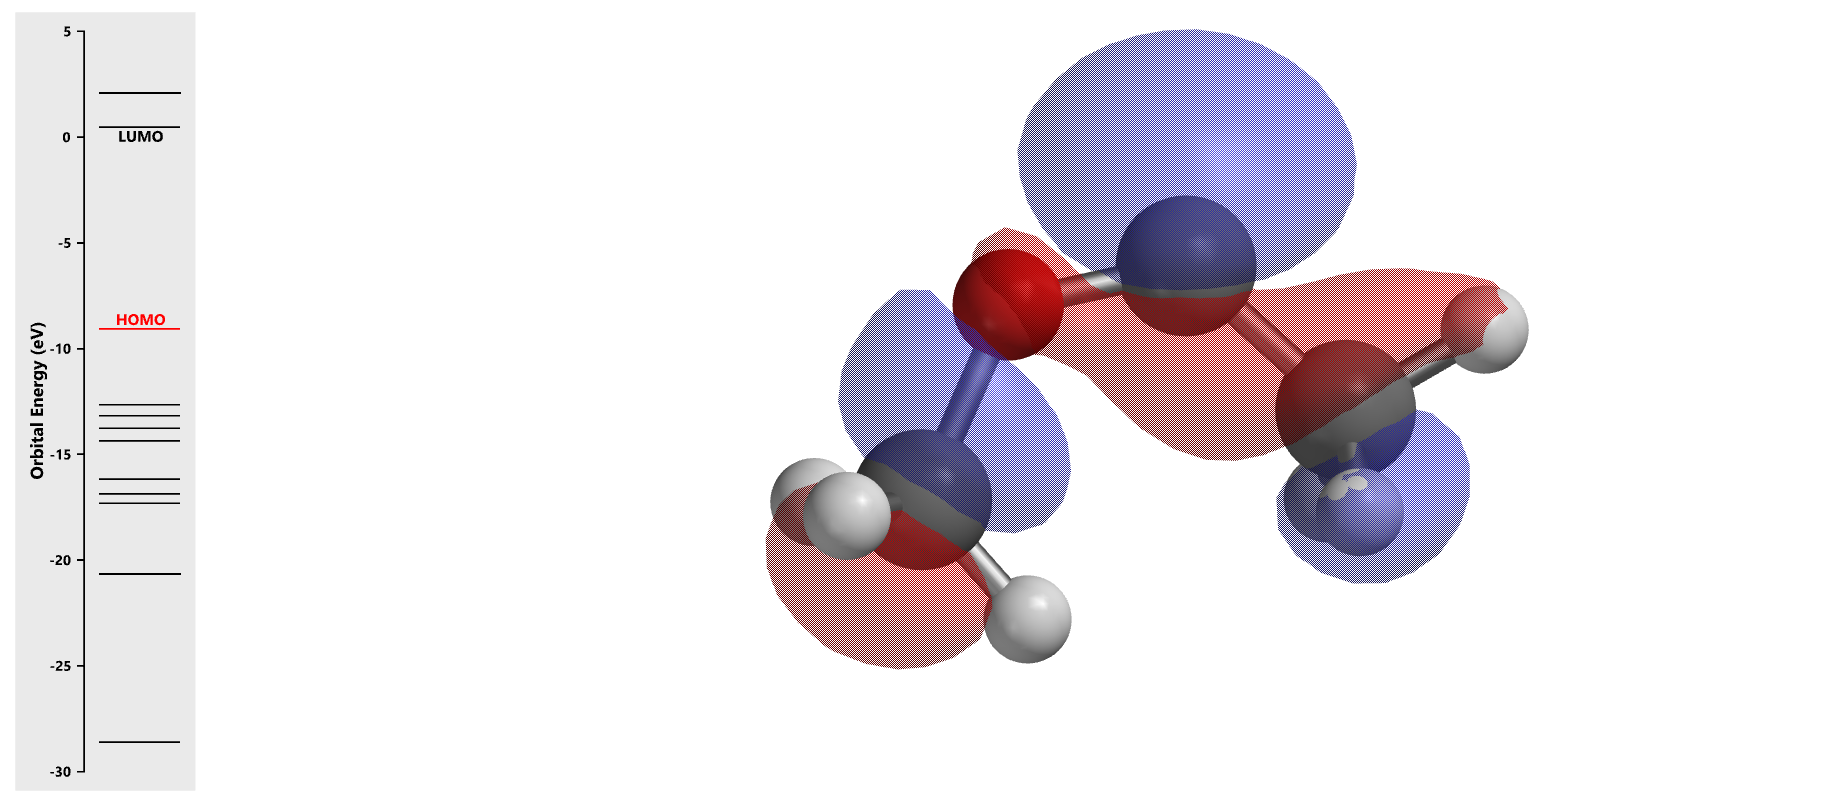
\includegraphics[width=0.95\columnwidth]{C(OMe)Me HOMO white background.png} %an example of how to make your figure a specific size (fraction of the width of the column), if you'd like it to span the column instead, delete the number before the \)
\vspace{2mm} %just an example of how space can be added if need be, replace with '\hspace' for horizontal padding
\caption{Same}
\end{figure}


The energy and C-O bond length of $Ph(OMe)CCr(CO)_5$ in four different structures were recorded in Table 3. The syn-conformation had lower energy than the anti-conformation, and the eclipsed form had lower energy than the staggered form. The syn-eclipsed structure had the lowest energy, meaning that the molecule was most stable under this structure. 

\begin{table}[h]
\caption{The energy of  $Ph(OMe)CCr(CO)_5$ in four different structures}
\begin{tabular}{L{1.0in}C{1.0in}C{1.0in}}\toprule
Conformation & Syn     & Anti    \\ \hline
Eclipsed     & -774.75 kJ/mol & -751.85 kJ/mol\\
Staggered    & -772.83 kJ/mol & -755.68 kJ/mol \\\bottomrule
\end{tabular}
\end{table}

The charge of the central carbon of $Ph(OMe)CCr(CO)_5$, $Ph(NH_2)CCr(CO)_5$, $TaCp_2Me(CH_2)$, and $TaCp_2Me(CH_2)AlMe_3$ were recorded in Table 4. For Fischer carbene (-C(OMe)Me) molecule, the charge of the central carbon was less positive as the -OMe group was replaced by -$NH_2$ group, meaning it is less electrophilic. For Schrock (-$CH_2$) carbene, the charge of the central carbon become less negative, which indicates that the carbon become less nucleophilic when $AlMe_3$ was added to the central carbon. 

\begin{table}[h]
\caption{The charge of the central carbon of Fischer and Schrock carbenes}
\begin{tabular}{L{1.5in}C{1.5in}}\toprule
Name of the molecules  & electrostatic (eV)    \\ \hline
 $Ph(OMe)CCr(CO)_5$    &  \\
$Ph(NH_2)CCr(CO)_5$     &  \\
$TaCp_2Me(CH_2)$     &  \\
$TaCp_2Me(CH_2)AlMe_3$ & \\\bottomrule
\end{tabular}
\end{table}


%\begin{figure}[h]
%  \centering
%  \subfloat[Flower one.]{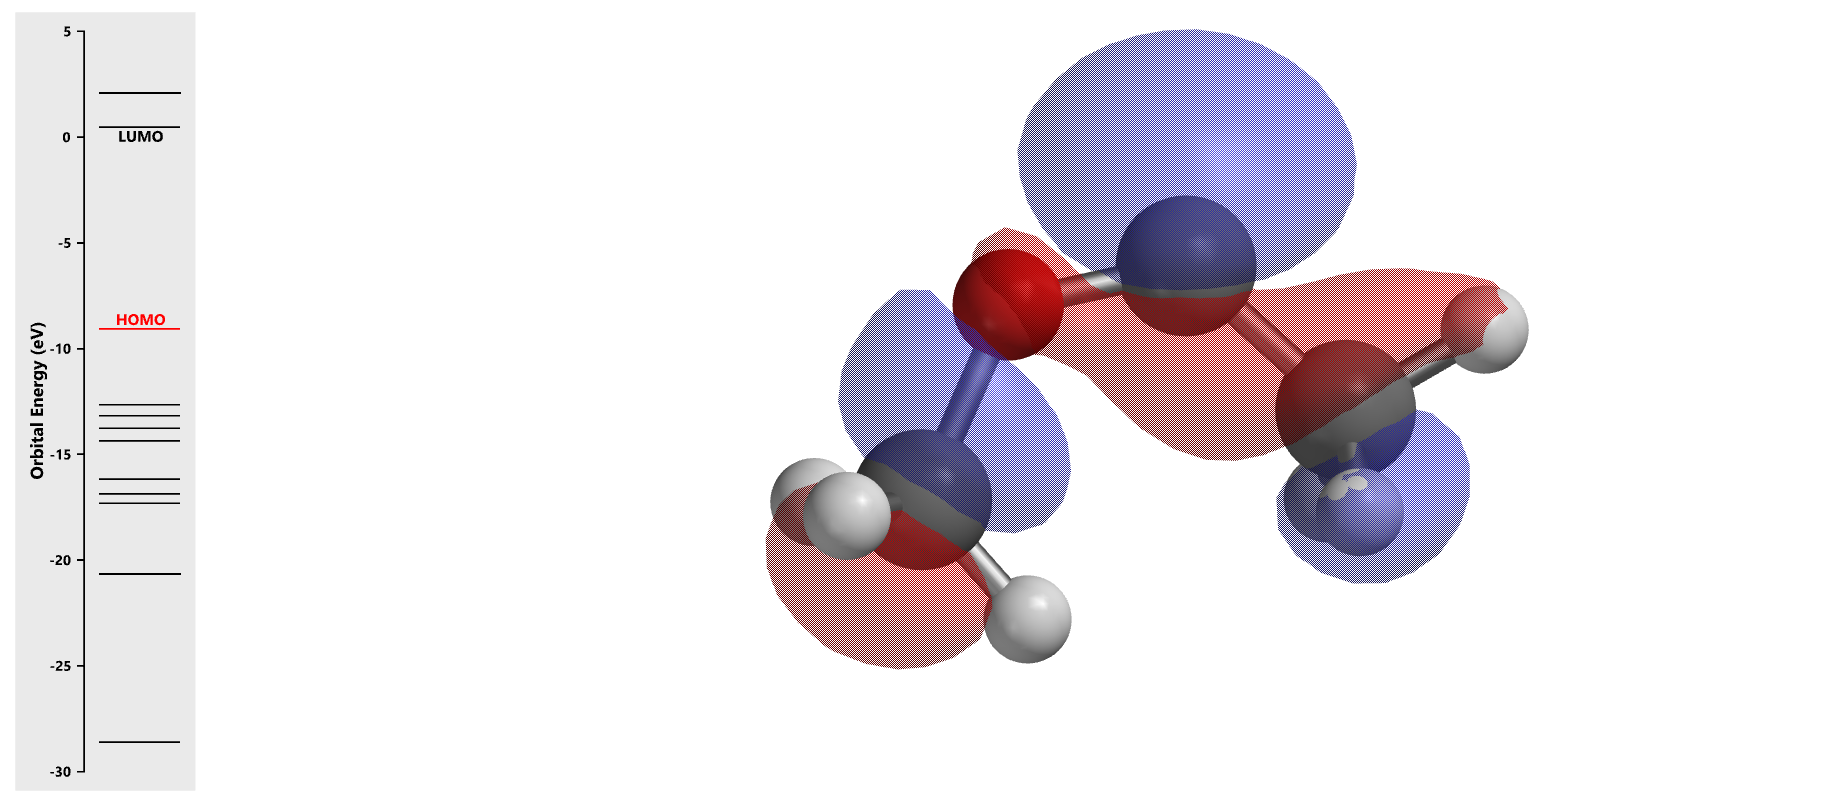
\includegraphics[width=0.95\columnwidth]{C(OMe)Me HOMO white background.png}\label{fig:f1}}
%  \hfill
%  \subfloat[Flower two.]{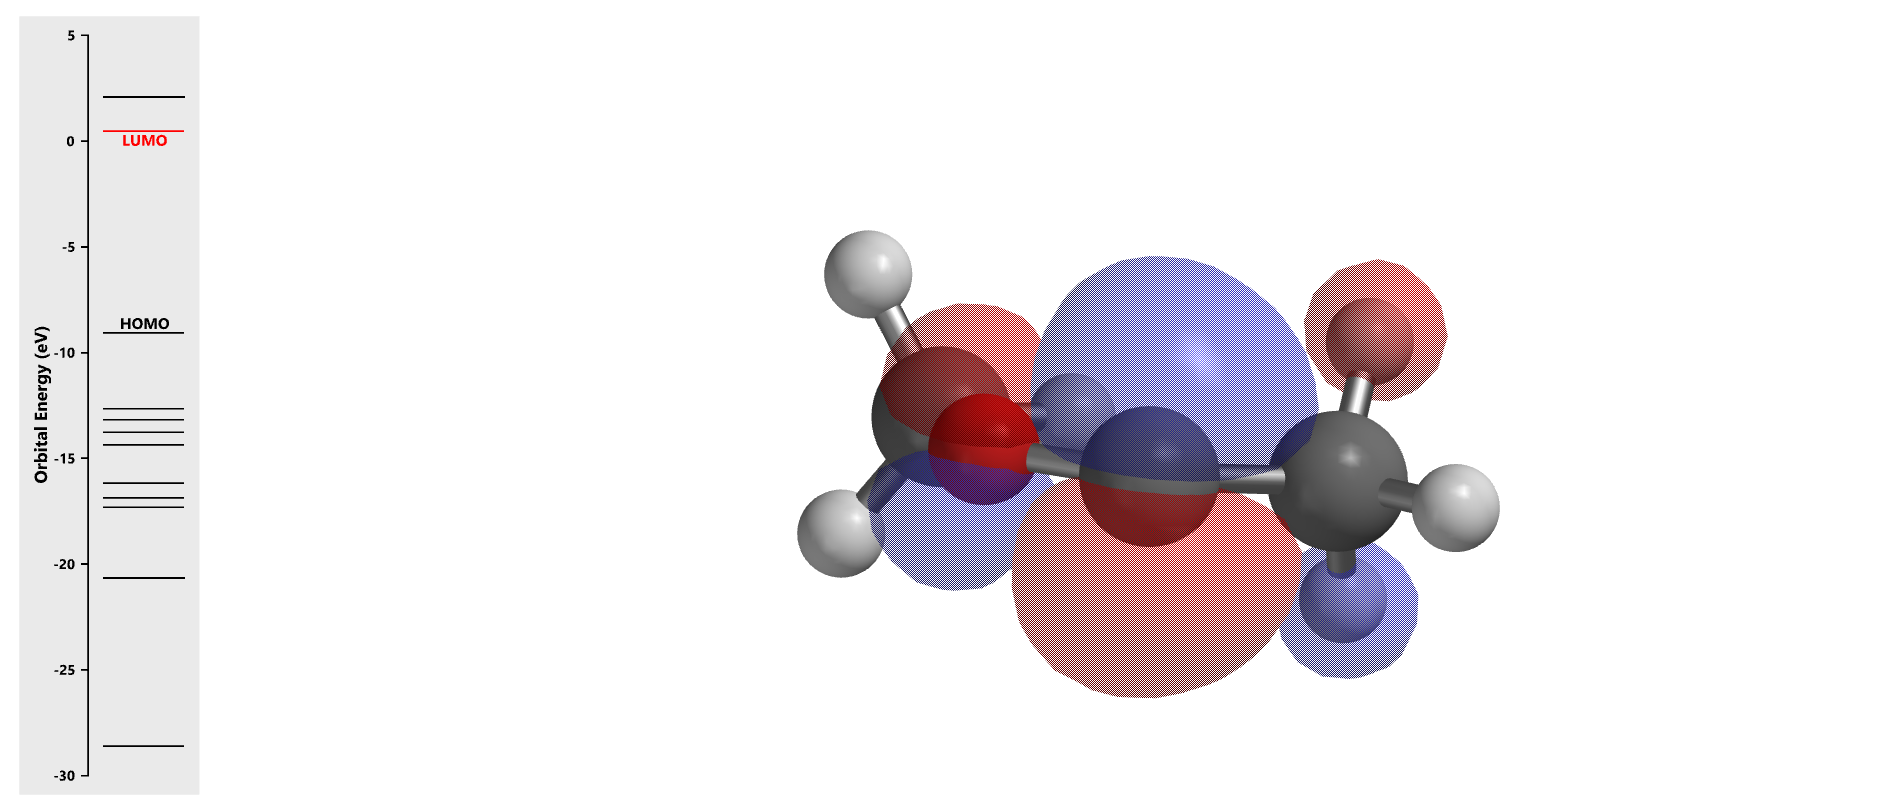
\includegraphics[width=0.95\columnwidth]{C(OMe)Me LUMO white.png}\label{fig:f2}}
%   \subfloat[Flower .]{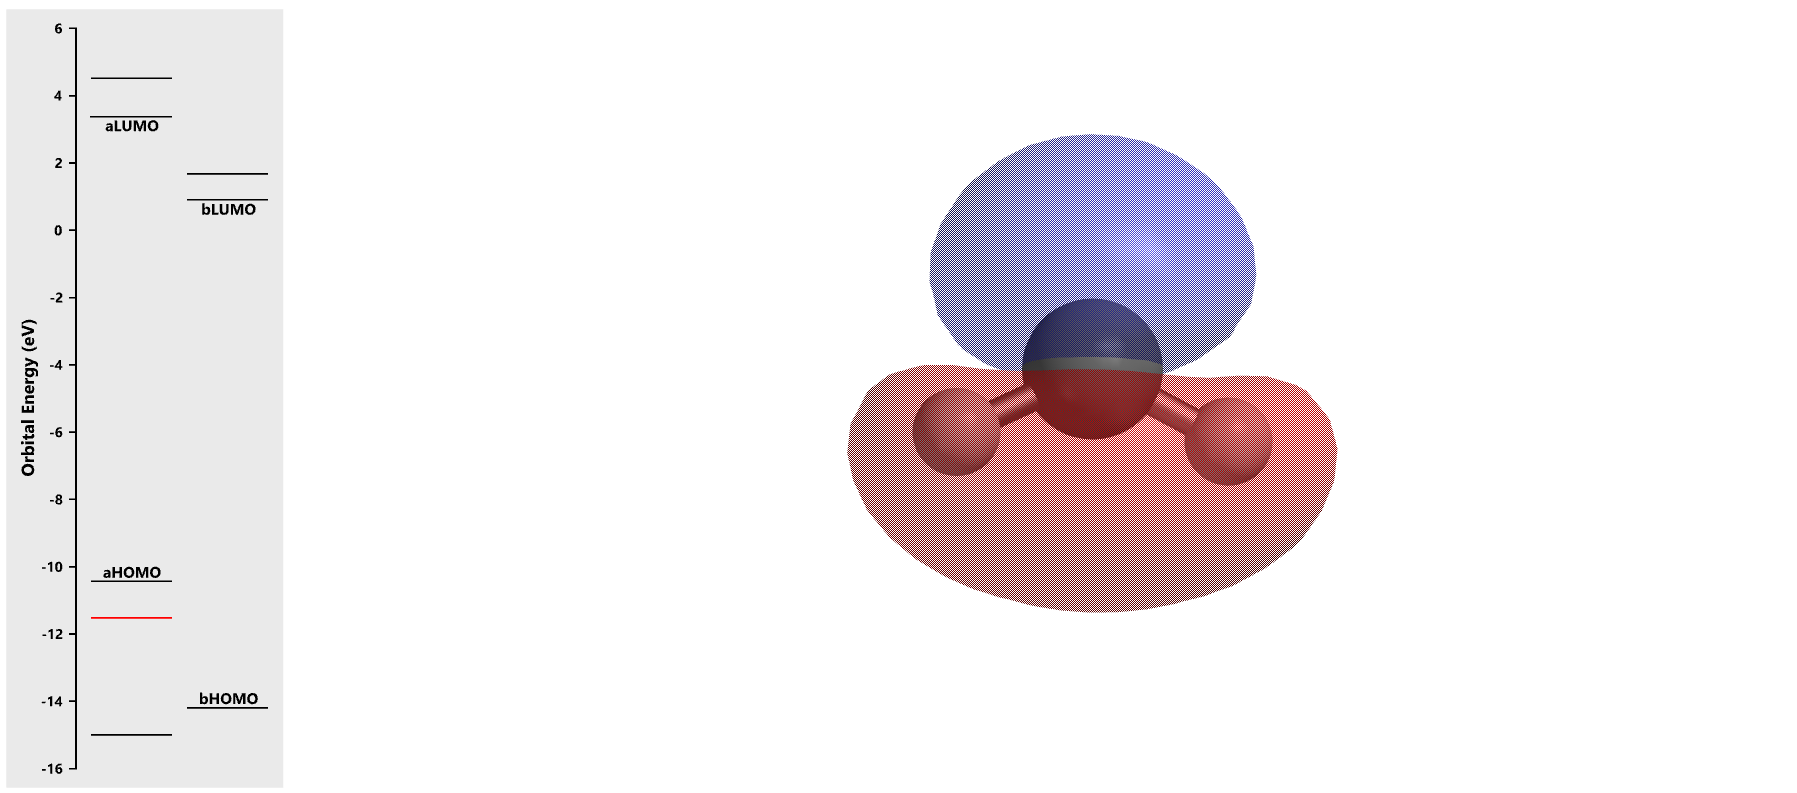
\includegraphics[width=0.95\columnwidth]{CH2 HOMO-1.png}\label{fig:f3}}
%  \caption{pictures with citation \cite{Montgomery}.}
%\end{figure}

%Be mindful that LaTeX -- unlike MS Word/Open Office/etc. -- does not allow for tables breaking across a page, by default. If the table is too big to fit into the remaining space of a page/column, it will instead be moved to the top of the following page/column. The resulting "empty" space will be filled with text, even if the text belongs to a different section! There are ways to prevent this, if you wish, but you may have to Google/look up how table formatting works :)



Please make sure you describe the data, particularly any trends that are apparent -- always avoid data-dumps. The best result section will guide the reader through the data, pointing out any important trends, values, or possible errors.

\bigskip %this is a way to force LaTeX into inserting a blank line/space, can be small, medium, or fixed by instead using the '\vspace' command!

If you wish to learn more about how to format tables, please visit \href{https://es.overleaf.com/learn/latex/Tables}{\textbf{this page}}.
You can also find a handy tool which can generate tables for you here: \url{https://www.tablesgenerator.com/}




\section{Discussion}
\textbf{Part 1}

The activation energy needed for inversion varies among different molecules. 

1. Nature of the central atom\\
$N^iPr_3$ vs. $P^iPr_3$\\

2. Substituent Effect\\
$PBr_3$ vs. $PF_3$ vs. $PCl_3$\\

3. Steric effect\\
$PPhMe_2$ vs. $PPhMe^tBu$\\

4. Conjugation effects\\
$P(C_6H_11)Me^nPr$ vs. $PPhMe^nPr$\\

5. Ring strain effects\\



\textbf{Part 2}

The energy of a triplet Fischer ligand ($C(OMe)Me$) was higher than the energy of its singlet form as shown in \textbf{Table x}, meaning that it was more stable for a Fischer molecule to stay in a singlet form. Thus, the ground electronic state of Fischer ligands were singlet states instead of triplet states. However, for a Schrock ligand ($CH_2$), the energy of its triplet state was lower than its singlet states, meaning that triplet states is more stable for Schrock ligands. Therefore, the ground electronic state of Schrock ligands is triplet states. 
The molecular orbital diagram of both $CH_2$ and $C(OMe)Me$ were shown in the \textbf{Figure x}. As $CH_2$ was a triplet, the energy of the two highest occupied molecular orbitals (HOMO)  were very close, so the stablest structures 

\\

\\
\\

\textbf{This again compares well with the experimental crystal structure of [Cr(CO)5(C(OMe)Ph)], which adopts this same geometry.}


%Here is an example of a figure.
%\begin{figure}[h!]
%\centering
%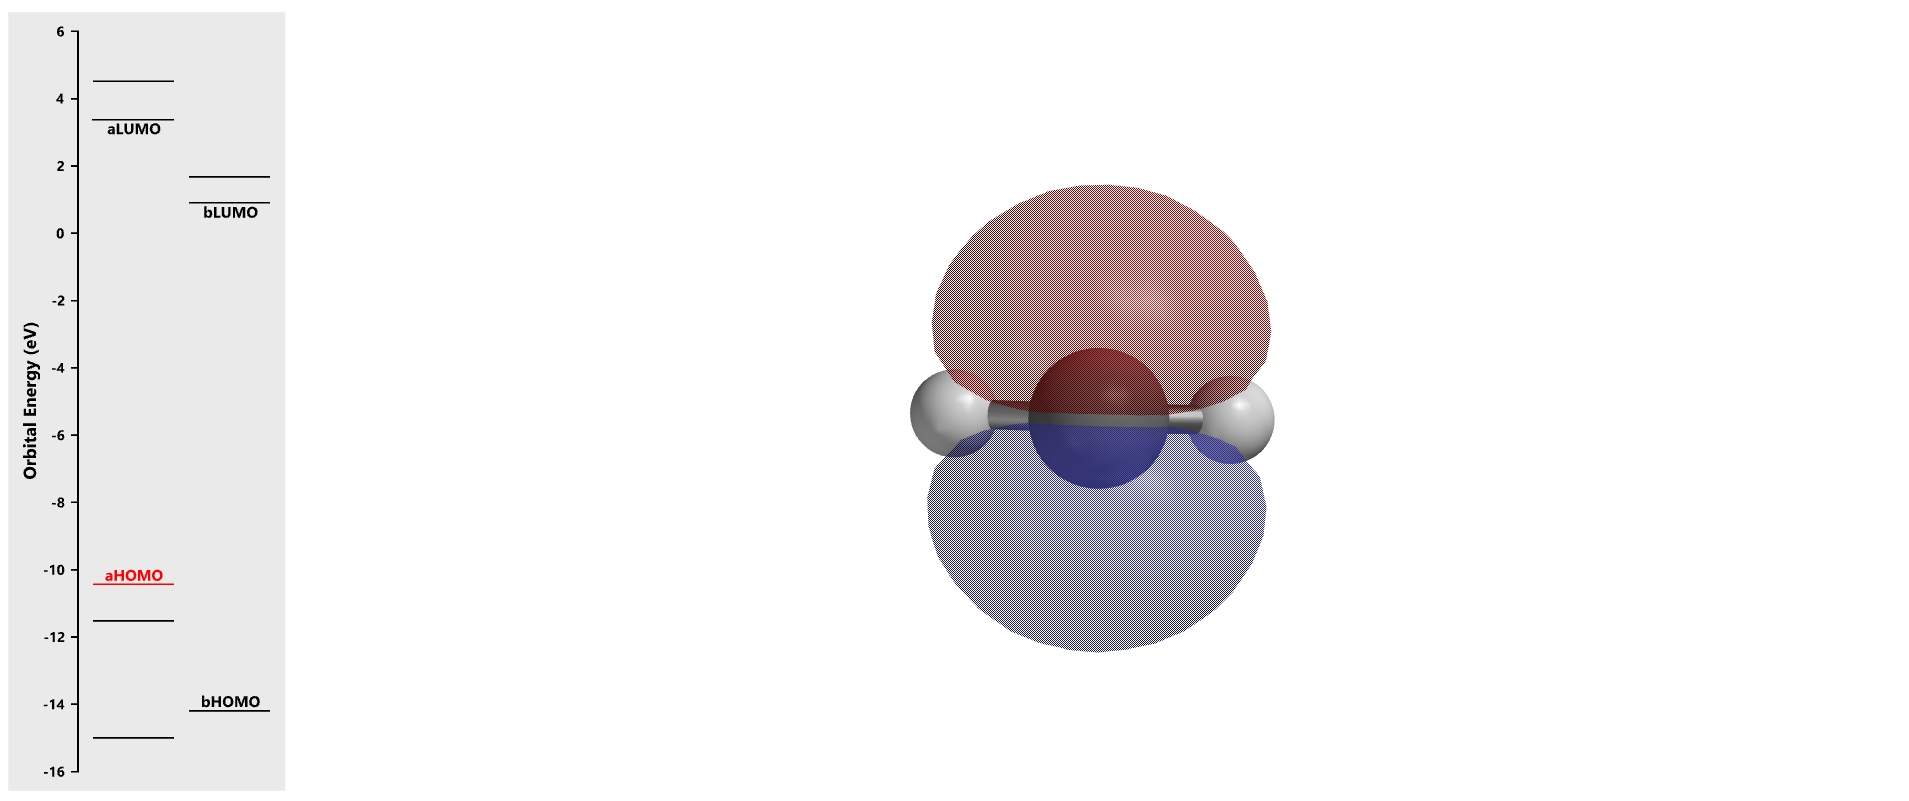
\includegraphics[width=0.95\columnwidth]{CH2 HOMO.png} %an example of how to make your figure a specific size (fraction of the width of the column), if you'd like it to span the column instead, delete the number before the \)
%\vspace{2mm} %just an example of how space can be added if need be, replace with '\hspace' for horizontal padding
%\end{figure}




\begin{figure}[h!]
\centering
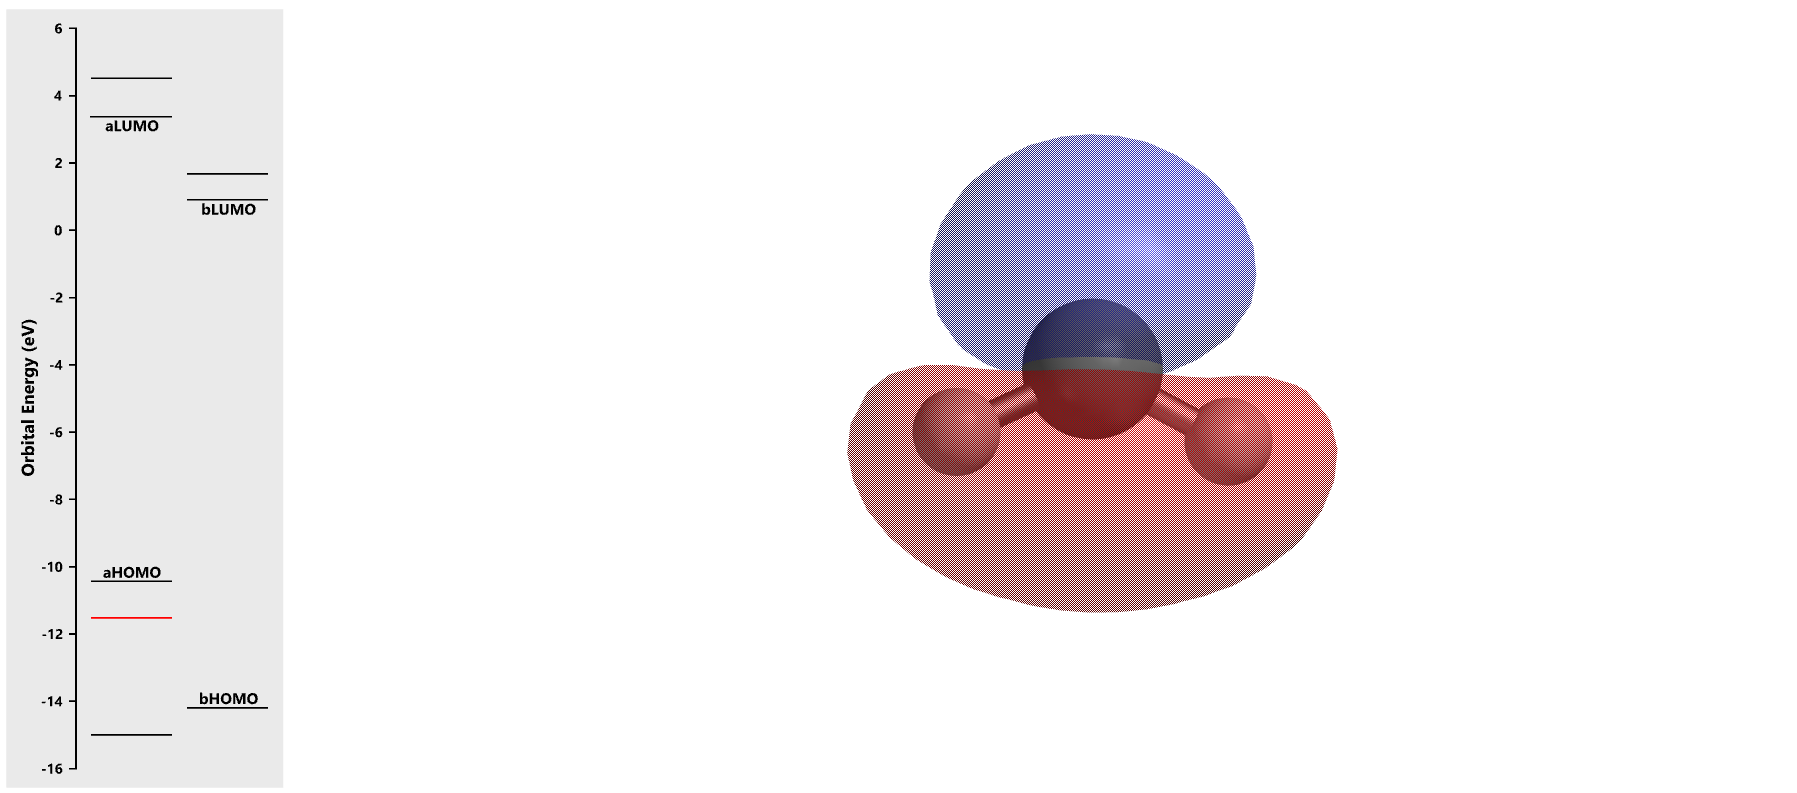
\includegraphics[width=0.95\columnwidth]{CH2 HOMO-1.png} %an example of how to make your figure a specific size (fraction of the width of the column), if you'd like it to span the column instead, delete the number before the \)
\vspace{2mm} %just an example of how space can be added if need be, replace with '\hspace' for horizontal padding
\caption{Same}
\end{figure}

Make use of figures and/or external references to support your discussion points. An example figure is shown above as Figure 1.

The best discussion will also include a brief paragraph with conclusions (for each part of the experiment) and future work. Future work, in this case, refers to a brief discussion on the validity of your chosen method, and the justification of using computational methods for the purposes of this experiment. The best discussion will offer some suggestions on the improvement of the experimental design.

\textbf{Please use concise and scientific tone in your writing. Academic writing, by convention, uses the past tense and a passive voice. Try to emulate the style you see in textbooks/papers. Avoid the use of first (I/we) or second (you) person, informal language, overuse of conjunctions and pronouns (especially 'this/that'). Make sure to proofread and spellcheck your work before submitting!}

Again, if you aren't sure what is appropriate for academic writing, please consult the many guides available online, such as \href{https://libguides.reading.ac.uk/writing/style}{\textbf{this one}}





\section{Investigation Question}

Please include the write-up to your investigation question here. Include any relevant figures, sources, or background information, as instructed in your manual.
\\
The best Investigation Question will include:
\\1) a short, relevant introduction to the problem,
\\2) a clear and well-worded proposal of a solution (hypothesis), and 
\\3) a concise and well-researched backing/explanation for the solution. 

Use appropriate scientific language and make sure to properly reference all of your sources!

\vspace{8mm}
\hrule

%% THE FOLLOWING SECTIONS CONTAIN SOME ADDITIONAL INFORMATION FOR YOUR CONVENIENCE, MAKE SURE TO REMOVE THEM FROM YOUR OWN REPORT %%

\section*{Note on the Citation} %Delete this section in your own report
All sources should be formatted in the Royal Society of Chemistry (RSC) referencing style \cite{Example}. If you don't know what this means, I strongly recommend reviewing how citation and referencing works in general, and looking into the style guides for the RSC style in particular. 
%more info at https://edu.rsc.org/download?ac=14556  

If you use a different referencing style (MLA, Harward, etc.) please indicate so in a footnote\footnote{Example on how to format a footnote in \LaTeX{}} of your citation section, so that the demonstrator marking your work knows that you've used something different and can check it for errors!

With Overleaf, you can simply import a .bib file into your file tree (the panel on the left-most side of your screen) and the bibliography command will automatically compile them for you. Please make sure to include relevant in-text references using the \textbackslash cite command.
The \textbackslash printbibliography command will then generate the proper references section for you!

.bib file can be easily obtained using a reference-management software. If you don't know what this is, or don't yet use one, I \textbf{strongly} recommend looking into one! Personally, I use \href{https://www.mendeley.com/reference-management/reference-manager}{Mendeley}, which has both a desktop version and a browser plug-in — this enables you to add references as you browse/research. If you learn how to use a reference management software now, it will save you tons of time later on; while you're writing your thesis, or other works in the future.

Further guidelines on referencing in LaTeX can be found here:
\url{https://www.overleaf.com/learn/latex/Bibliography\_management\_in\_LaTeX}

\section*{Tips and Tricks} %make sure to delete this from your report!!

\LaTeX{} is a widely used compiler, there are hundreds of tutorial articles and videos online - please make use of them! Google is your friend, you need only ask.

% Sidenote from Angie: I'm (a bit) sorry for bullying you with Overleaf and LaTeX coding, but I promise if you give it a chance, you'll learn to love it :) it's very useful for writing larger pieces of academic writing ⁠— such as your future thesis! Plus, it is another shiny, new skill to spruce up your future CVs.

\subsection*{How to write Mathematics} %make sure to delete this from your report

\LaTeX{} is great at typesetting mathematics. Let $X_1, X_2, \ldots,
X_n$ be a sequence of independent and identically distributed random
variables with $\text{E}[X_i] = \mu$ and $\text{Var}[X_i] = \sigma^2 <
\infty$, and let
\[S_n = \frac{X_1 + X_2 + \cdots + X_n}{n}
      = \frac{1}{n}\sum_{i}^{n} X_i\]
denote their mean. Then as $n$ approaches infinity, the random
variables $\sqrt{n}(S_n - \mu)$ converge in distribution to a normal
$\mathcal{N}(0, \sigma^2)$.

\subsection*{How to add Lists} %make sure to delete this from your report

You can make lists with automatic numbering \dots

\begin{enumerate} %for numbered list
\item Like this,
\item and like this.
\end{enumerate}
\dots or like this, \dots
\begin{itemize} %for bullet points
\item Like this,
\item and like this.
\end{itemize}


%% I M P O R T A N T %%
%%!!!REFERENCES -- REVIEW FOR YOUR OWN REPORT!!!%%

\bibliography{example_refs} %This command generates your bibliography. PLEASE MAKE SURE TO CHANGE THE NAME IN THESE CURLY BRACKETS TO WHATEVER YOUR .BIB FILE IS CALLED!!
\bibliographystyle{rsc} %setting for the RSC's .bst (style) file -- do NOT change this, unless you wish to define a new citation style

\end{document}


%Best of luck with your report! 

%Last SideNote: If you have any questions ask them during the lab session, you should have plenty of time and opportunity to go over everything. If you need more help once your sessions are over and you can't figure something out yourself, you can contact me at angie.matusova@ed.ac.uk. Please, don't hesitate to get in touch if you're struggling with something (though, please make sure you've exhausted all the other options before contacting me; i.e. you've reviewed all the material available on Learn and/or tried looking up your query online).